\documentclass{article}
\usepackage{graphicx}
\usepackage{amsmath}
\usepackage{float}
\usepackage{amsfonts}
\usepackage{listings}
\usepackage{xcolor}
\usepackage[utf8]{inputenc}
\usepackage{hyperref}
\usepackage{fancybox}
\usepackage{booktabs}
\usepackage{array}
\usepackage{tikz}
\usepackage{amsfonts}
\usepackage{dsfont}
\usepackage{pgfplots}
\pgfplotsset{compat=1.18}
\usepackage[margin=2cm]{geometry}
\usepackage[french]{babel} % Pour les éléments en français
\usetikzlibrary{shapes, arrows.meta, positioning}
\usepackage[labelfont=bf, font=small]{caption}  % Pour personnaliser le titre de la figure


\title{TP2 ADM Classification automatique}
\author{SCAIA Matteo et MARIAC Damien}
\date{\today} 

\begin{document}

\maketitle

\begin{figure}[h] 
    \centering
    
\includegraphics[width=0.5\textwidth]{ssd_logo.png} 
\end{figure}

\begin{figure}[h] 
    \centering
    
\includegraphics[width=0.5\textwidth]{logo_um_2022_rouge_RVB.png} 
\end{figure}

\newpage

\tableofcontents

\newpage
\section{Treillis de Galois}
\subsection{Introduction}
Le treillis de Galois est une structure mathématique utilisée en analyse de données pour extraire des règles d’implication. Il est construit à partir de données décrites par des propriétés booléennes, permettant de représenter les relations entre ces propriétés et les ensembles d’objets associés. 
Le treillis de Galois peut également intégrer des relations liant les données entre elles.
\subsection{Interprétation et création du treillis de Galois}
Dans cette question, nous allons analyser le treillis de Galois construit à partir des données fournies par le sujet afin de modéliser les relations entre les films et leurs caractéristiques.
\begin{figure}[h]
    \centering
    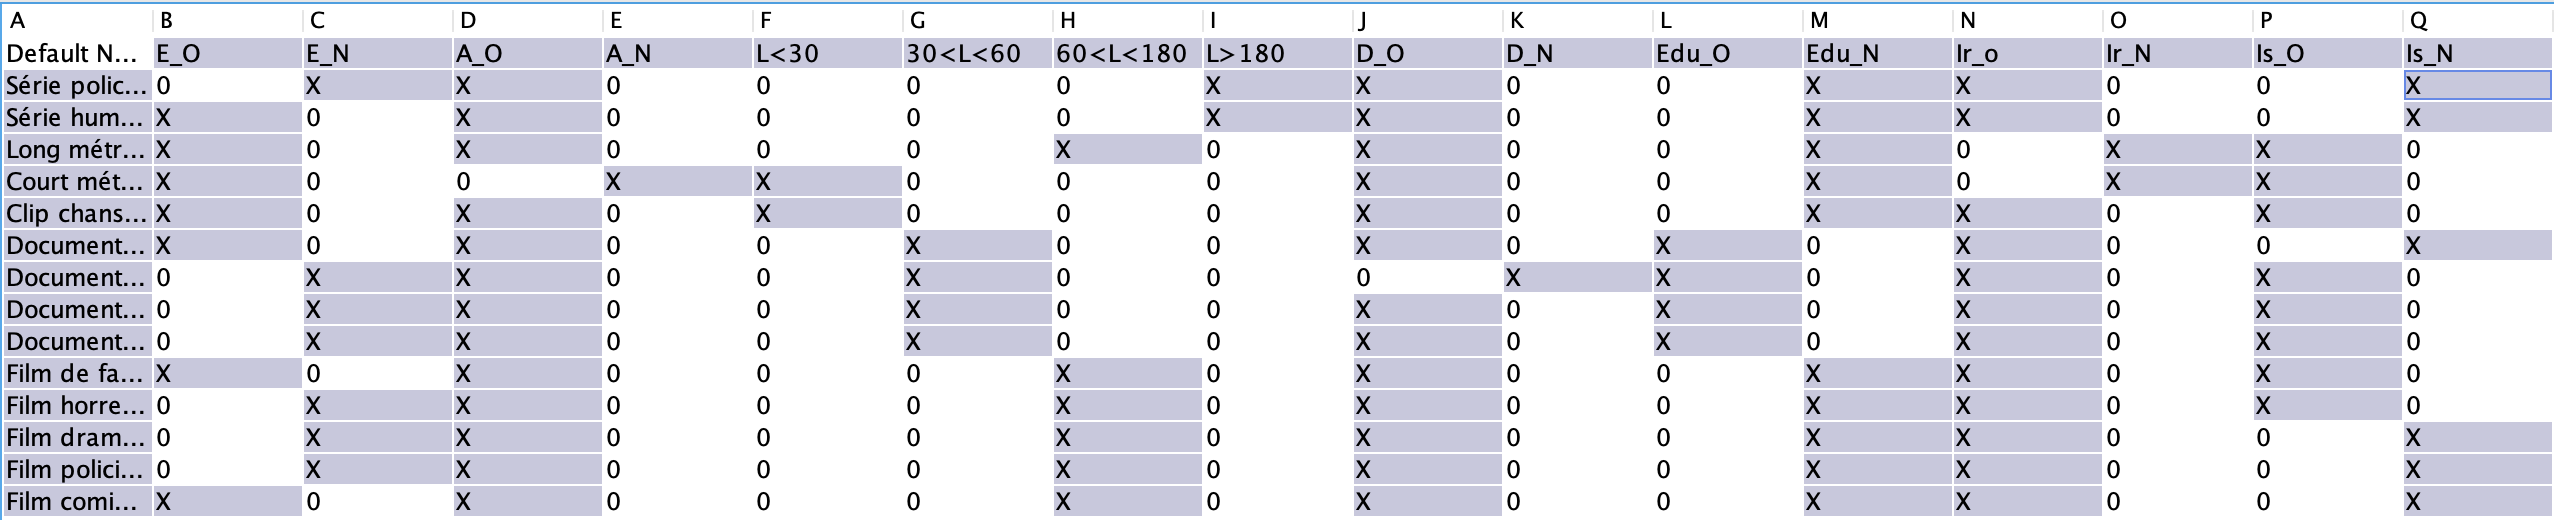
\includegraphics[width=0.7\textwidth]{tableau.png}
    \caption{Tableau des relations binaires}
    \label{fig:tableau} 
\end{figure}
\\
À l'aide du logiciel Galicia, nous obtenons le treillis de Galois suivant :
\begin{figure}[h]
    \centering
    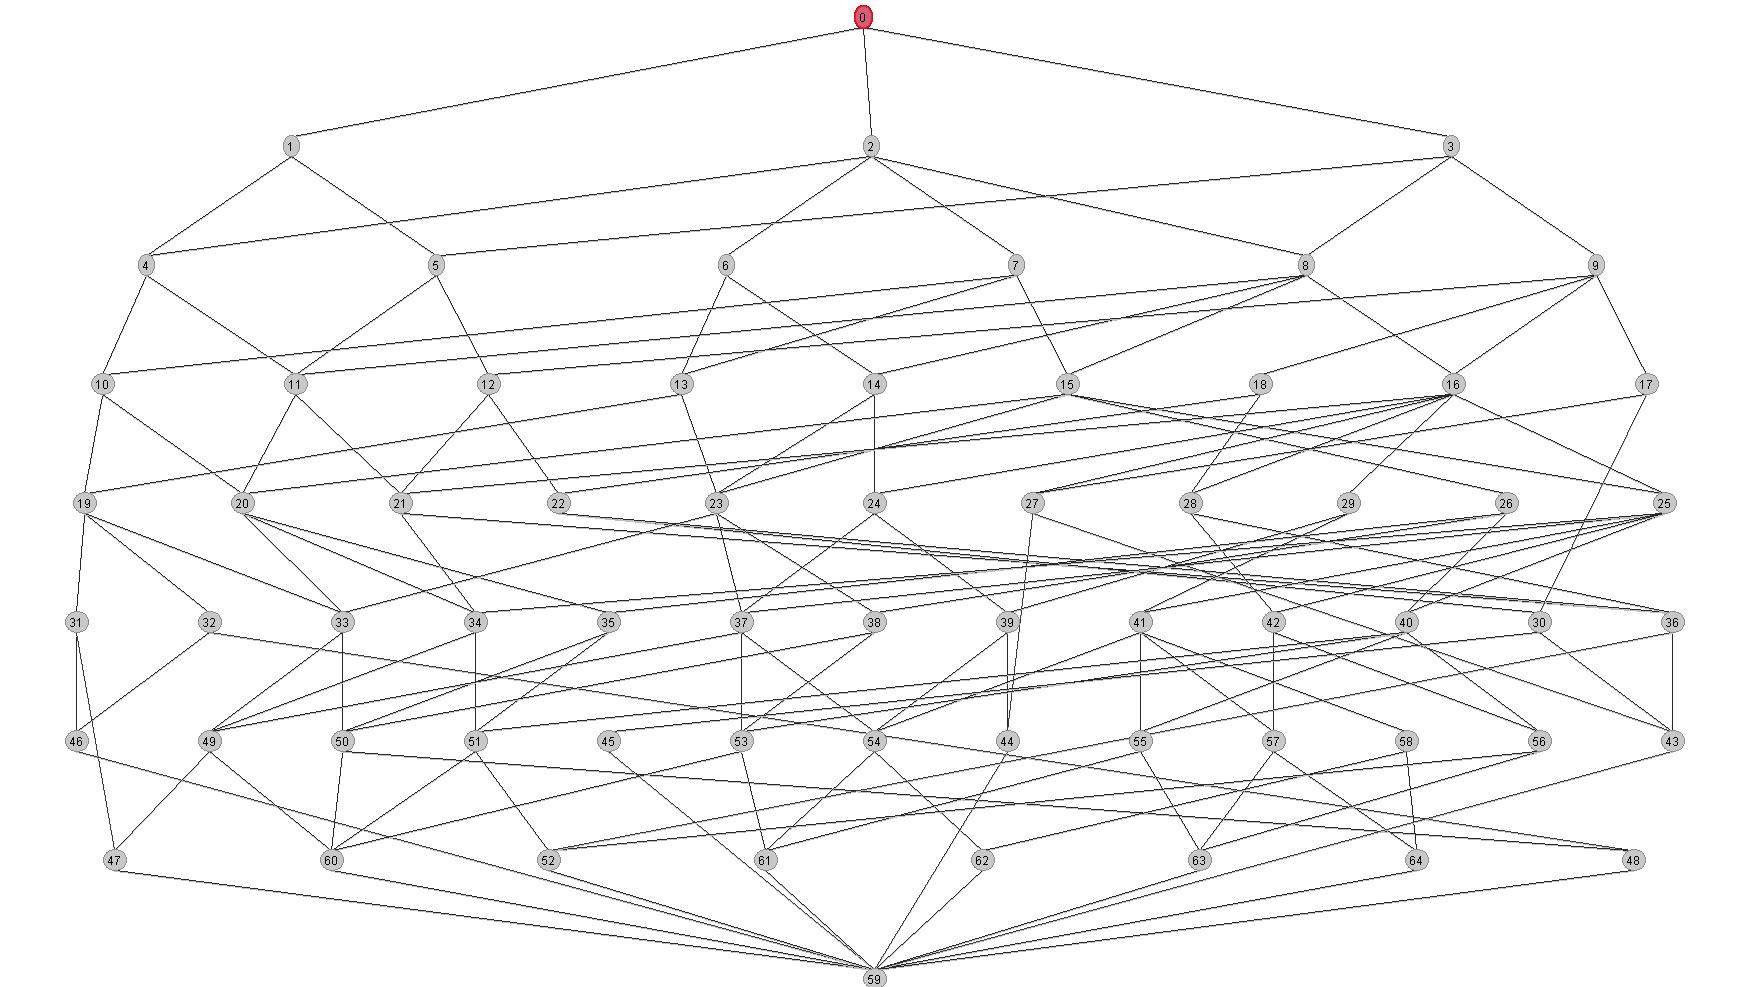
\includegraphics[width=0.7\textwidth]{treillis.png}
    \caption{Treillis de Galois de notre tableau}
    \label{fig:treillis} 
\end{figure}
\\
Dans un treillis de Galois, les nœuds situés aux extrémités correspondent soit à l’ensemble de tous les individus, soit à l’ensemble de toutes les caractéristiques. Ces nœuds étant trop généraux ou trop spécifiques, leur analyse n’est pas nécessaire. Nous concentrerons notre attention sur les nœuds possédant le plus grand nombre de connexions, car ils semblent jouer un rôle central en reliant plusieurs classes.
\end{document}